\chapter{Wstęp}
W dobie powszechnego dostępu do internetu i informatyzacji człowiek człowiek produkuje olbrzymie ilości danych.
Każdego dnia setki milionów ludzi robic zdjęcia, filmy i wysyła wiadomości tekstowe.
Rządy państw regularnie zbierają dane wszelkiego rodzaju, od spisów statysczynych po raporty incydentów od jednostek policji.
Ogrom tych danych rośnie w dużym tempie.
Całkowita liczba danych na świecie wyniosła 4.4 zettabajów ($4.4 * 10^{21}$) danych.
Prognozuje się dalszy wzrost do 44 zettabajtów do roku 2020.
Szacuje się, że dziennie powstaje ok. 2,5 exabajtów ($2,5 * 10^{18}$ bajtów) danych. \cite{khoso2016}
Z jednej strony jest to wyzwanie, gdyż aby przetwarzać tak wielką liczbę danych potrzeba wielu zasobów - sieciowych, obliczeniowych i magazynowych.
Jedno z centrum obliczeniowych (\textit{Data Center}) firmy \textit{Facebook} w miejscowości \textit{Prineville} w stanie \textit{Oregon} składa się z 4 buynków o łącznej powierzchni ok. $42000 m^2$.
Poniżej, na rys. \ref{fig:data_center} przedstawiono 8 szaf serwerowych (\textit{rack}), każda złożona z 32 serwerów i mogąca przechować 2 petabajty danych. \cite{lardinois2016}.
Na 42 tys. $m^2$ można rozmieścić wiele takich szaf, co w wyniku daje olbrzymie możliwośći, a to zaledwie jeden z wielu takich kompleksów na świecie.

\begin{figure}[h!tb]
	 \centering
	 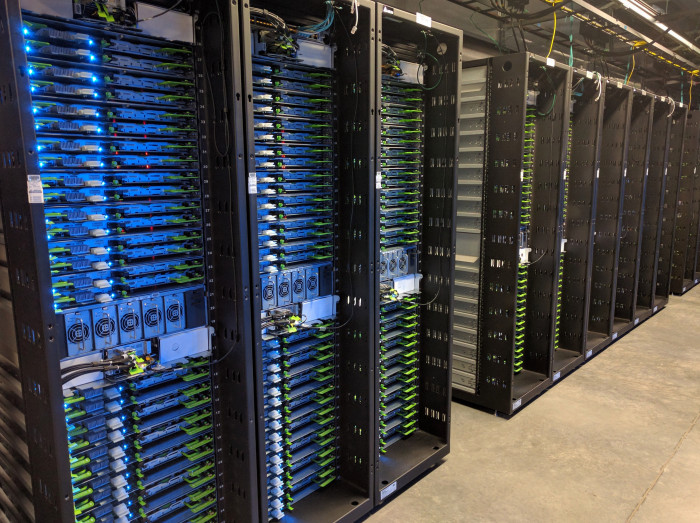
\includegraphics[width = 1.0\linewidth]{img/data_center}
	 \caption{Fragment centrum obliczeniowego \\
              Źródło: \cite{lardinois2016}}
	 \label{fig:data_center}
\end{figure}

Duża liczba danych niesie ze sobą zarówno wyzwania, jak i korzyści.
W ostatnich latach ukuło się w języku angielskim pojęcie \textit{Big Data}, które definiujemy jako duże zbiory danych zarówno ze zbiorów tradycyjnych jak i cyfrowych, które są źródłem dla nowych odkryć i analiz. \cite{Arthur2013}.
Przetwrzanie i analiza owych zbiorów danych jest skomplikowana i czasochłonna dla człowieka, dlatego z pomocą przychodzą algorytmy z dziedziny sztucznej inteligencji, a konkretnie ich podzbiór związany z uczeniem maszynowym \textit{Machine learning}, zdefiniowany dalej w rozdziale \ref{chap:teoria}.
Typowymi zastosowaniem tego typu algortymów jest filtr antyspamowy, które klasyfikuje wiadomości jako spam na podstawie dużego zbioru wiadomości oznaczonych jako spam lub nie.
Innym popularnym zastosowaniem są systemy rekomendacji - za przykład niech posłuży system w odtwarzaczu \textit{Spotify}, który na podstawie słuchanej przez użytkownika muzyki dobiera dla niego propozycje, które również mogą mu się spobodać, ze względu na podobieństwo.
Przykładowe rekomendacje przedstawiono na rys. \ref{fig:recommendations}.

\begin{figure}[h!tb]
	 \centering
	 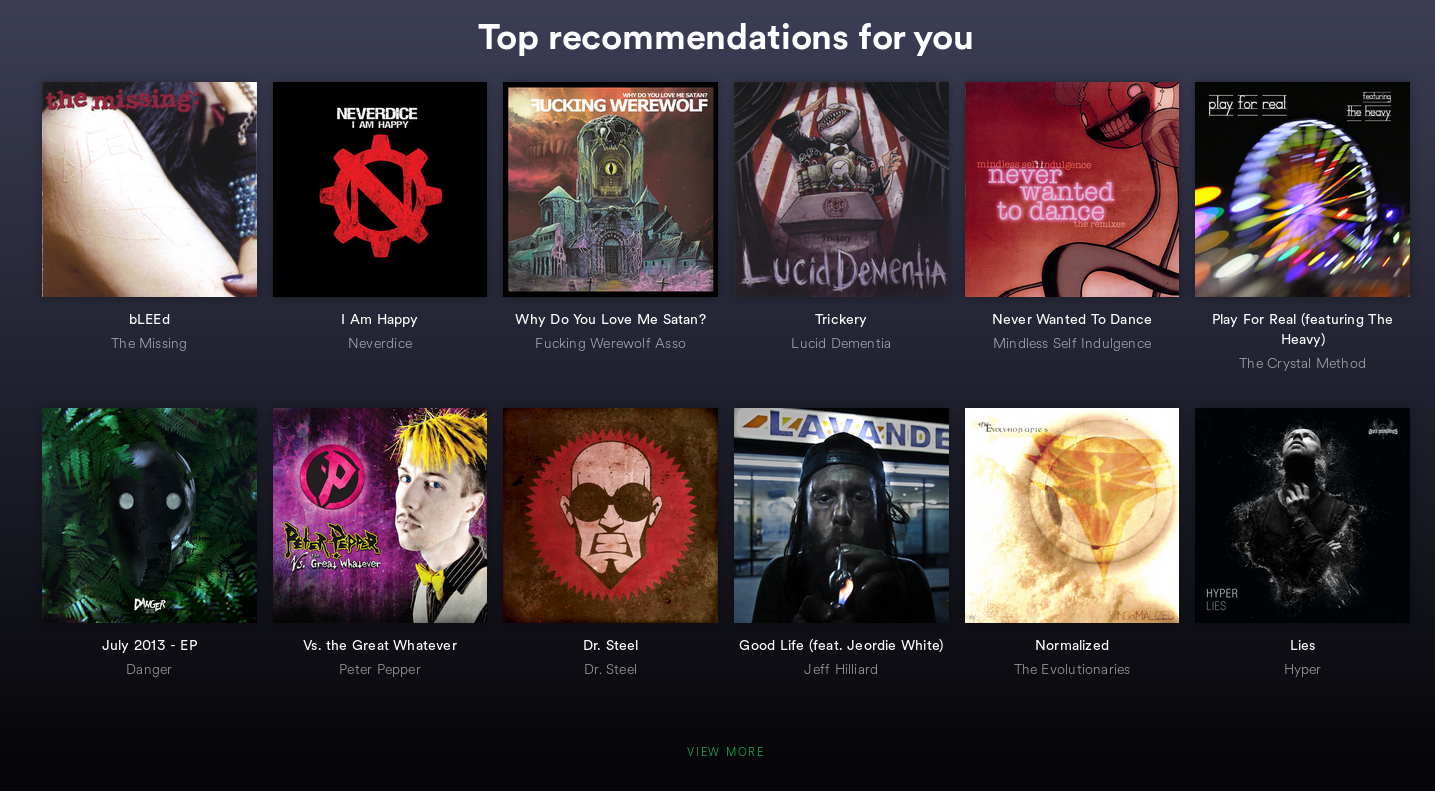
\includegraphics[width = 1.0\linewidth]{img/recommendations}
	 \caption{Rekomendowana przez algorytmy uczenia maszynowego muzyka w serwisie \textit{Spotify} \\
              Źródło: praca własna}
	 \label{fig:recommendations}
\end{figure}

Rozwiązania tego typu stosuje wiele innych popularnych serwisów multimedialnych, między innymi \textit{YouTube}, \textit{Netflix}.
Algorytmy tego typu, co zostanie przybliżone w rozdziale \ref{chap:teoria}, uczą się na podstawie podanych im danych, każdy jednak taki algorytm (np. sieci neuronowe), opisać można przez kilka parametrów.
Parametry owe można dobierać w sposób arbitralny, można jednak również do wyznaczania ich optymalnych nastaw zaprząc inny algorytm (należący również klasy algorytmów SI lub nie), np. algorytm genetyczny, algorytmy roju itd..
Inspiracją do przeprowadzenia badań w tym kierunku były zajęcia laboratoryjne z przedmiotu Sztuczna Inteligencja w Automatyce na studiach inżynierskich na kierunku Automatyka i Robotyka na wydziale Elektroniki, Telekomunikacji i Informatyki Politechniki Gdańskiej.
Jedno z zadań laboratyjnych polegało na znalezieniu optymalnych parametrów sieci neuronowej, tak aby wynikowa sieć dobrze aproksymowała zadaną funkcję.
Korzystając z pewnej wiedzy na temat samych sieci neuronowych oraz dobierania liczby neuronów, rodzaju funkcji aktywacji, liczby warstw ostatezcnie metodą prób i błędów dochodziło się do zadowalającego rozwiązania.
W tym miejscu pojawiła się idea, aby nie robić tego ręcznie, a użyć innego algorytmu.
Stąd wysunąć można główną tezę tej pracy - że możliwa jest opytamlizacja owych parametrów za pomocą algorytmu genetycznego.
Dodatkowo, w związku z tym, że pełne uczenie większych sieci dla bardziej skomplikowanych problemów jak klasyfikacja obrazów jest czasochłonne, poszukiwano sposobu na skrócenie owego czasu.

Poprzez analogię do świata ludzi, gdzie można dla wielu przypadków zaobserwować prawidłowość, że mądre dzieci szybko się uczą i ostatecznie dochodzą do lepszych wyników jako dorośli, niż dzieci mniej rozgarnięte, wysnuto dodatkową tezę, mianowicie, że istnieje związek pomiędzy wynikami danej sieci neuronowej po uczeniu przez jedną epokę a jej finalną skutczenością po uczeniu pełnym.
Dalej przedstawiony zostanie przegląd stanu wiedzy w rozdziale \ref{chap:teoria}, zostanie opisany system, który powstał w celu udowodnienia owych tez w rozdziale \ref{chap:system_description} oraz omówione zostaną wyniki badań w rodziale \ref{chap:tests}.
Wszystko zostanie podsumowane w rozdziale \ref{chap:summary}.
